\renewcommand{\chaptername}{March 8th: Lab}
\chapter{Qubits and Quantum Circuits}
%rotate the STATE? or QUBIT?
%centre captions

Conventionally, information is stored in bits, as a series of 0s and 1s. However, in quantum computing `quantum bits', or simply `qubits', are used. These obey the rules of quantum mechanics and allow for information to be processed in new and different ways.

In order to manipulate these qubits (i.e. change them between quantum states) `quantum gates' can be applied to build a 'quantum circuit'. A quantum circuit is a computational routine consisting of coherent quantum operations on quantum data, such as qubits, and concurrent real-time classical computation. It is an ordered sequence of quantum gates, measurements and resets, all of which may be conditioned on and use data from the real-time classical computation.

\section{Objectives}
The purpose of this lab is to investigate quantum bits and quantum circuits using IBM's `qiskit`. Thus, the following objectives were pursued:
\begin{itemize}
    \item Become familiar with `qiskit'
    \item Implement quantum gates and visualise the state of a qubit through the Bloch sphere
    \item Obtain deeper understanding of quantum operations and quantum circuits basics
\end{itemize}

\section{Methods}
Quantum circuits were implemented and visualised using python in Jupyter Notebook -- a web-based interactive computational environment for programming languages. Specifically, a library named `qiskit' was used -- an open-source software development kit for working with quantum computers. It provides tools for creating quantum programs and for running them on simulators on a local computer. The Aer simulator was used; this provides high-performance quantum computing simulators with realistic noise models locally, and visualization allows you to see what you states look like

To evaluate the rigidity of the analytical predictions from qiskit, the circuits were built on protoype quantum devices provided by IBM Quantum. `The IBM Quantum Composer' is an online platform allowing public access to remote quantum computing services.

%Reference screenshots of code

\section{Results}
Qubits can be represented by 2D vectors, their states are limited to the form:

$$ |q\rangle = \cos{\tfrac{\theta}{2}}|0\rangle + e^{i\phi}\sin{\tfrac{\theta}{2}}|1\rangle $$
where $\theta$ and $\phi$ are real numbers. 

This state can be visualized using a `Bloch Sphere' (a geometrical representation of a two-level qubit) and quantum gates can be used to manipulate the state. An important feature of quantum circuits is that quantum gates are always reversible. These reversible gates can be represented as matrices, and as rotations around the Bloch sphere.

In this lab report, Pauli gates, the Hadamard gate and some Multi-qubit gates are analysed in detail.

\subsection{The Pauli Gates}
Pauli matrices can represent some commonly used quantum gates. 

\subsubsection{The X Gate}
The X gate is represented by the Pauli-X matrix:

$$ X = \begin{bmatrix} 0 & 1 \\ 1 & 0 \end{bmatrix} = |0\rangle\langle1| + |1\rangle\langle0| $$

A circuit was created to determine the effect an X gate has on a qubit. A qubit was initialised in state $|0\rangle$ and was passed through an X gate, the circuit diagram of which is shown in Figure \ref{fig:xGate}.

\begin{figure}[h]
    \centering
    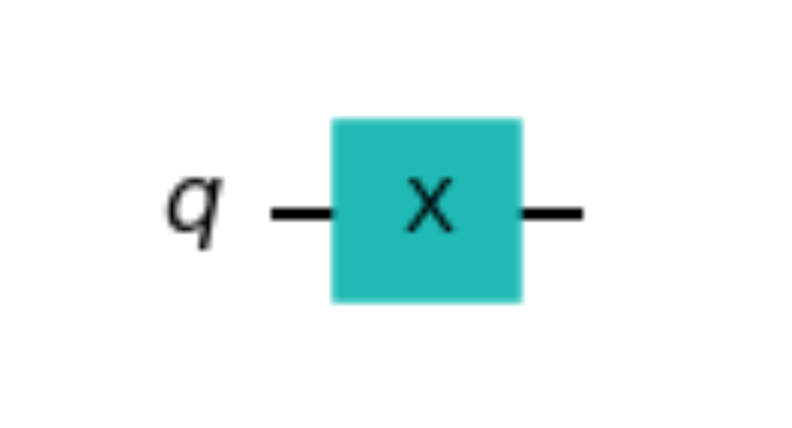
\includegraphics[width=0.3\textwidth]{lab2/images/xGate.png}
    \caption{Circuit diagram of a Pauli-X gate} 
    \label{fig:xGate}
\end{figure}

From the mathematics, it is clear that applying an X gate switches the amplitudes of the states $|0\rangle$ and $|1\rangle$:

$$ X|0\rangle = \begin{bmatrix} 0 & 1 \\ 1 & 0 \end{bmatrix}\begin{bmatrix} 1 \\ 0 \end{bmatrix} = \begin{bmatrix} 0 \\ 1 \end{bmatrix} = |1\rangle \quad\quad\quad\quad
X|1\rangle = \begin{bmatrix} 0 & 1 \\ 1 & 0 \end{bmatrix}\begin{bmatrix} 0 \\ 1 \end{bmatrix} = \begin{bmatrix} 1 \\ 0 \end{bmatrix} = |0\rangle$$

%DEMONSTRATED
The circuit in Figure \ref{fig:xGate} was implemented in X and the states were obeserved using a Bloch sphere. Figure \ref{fig:bSphereXGate} shows the X gate performs a rotation by $\pi$ around x-axis of the Bloch sphere (the qubit switched to state $|1\rangle$ after being initialised in state~$|0\rangle$).

\begin{figure}[h]
    \centering
    \begin{subfigure}[h]{0.33\textwidth}
        \centering
        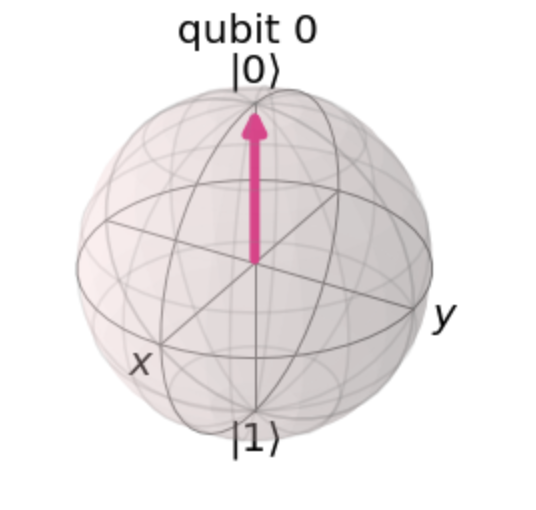
\includegraphics[width=\textwidth]{lab2/images/bSphX1.png}
        \caption{}
        \label{fig:bSphX1}
    \end{subfigure}
    \hspace{0.2\textwidth}
    \begin{subfigure}[h]{0.33\textwidth}
        \centering
        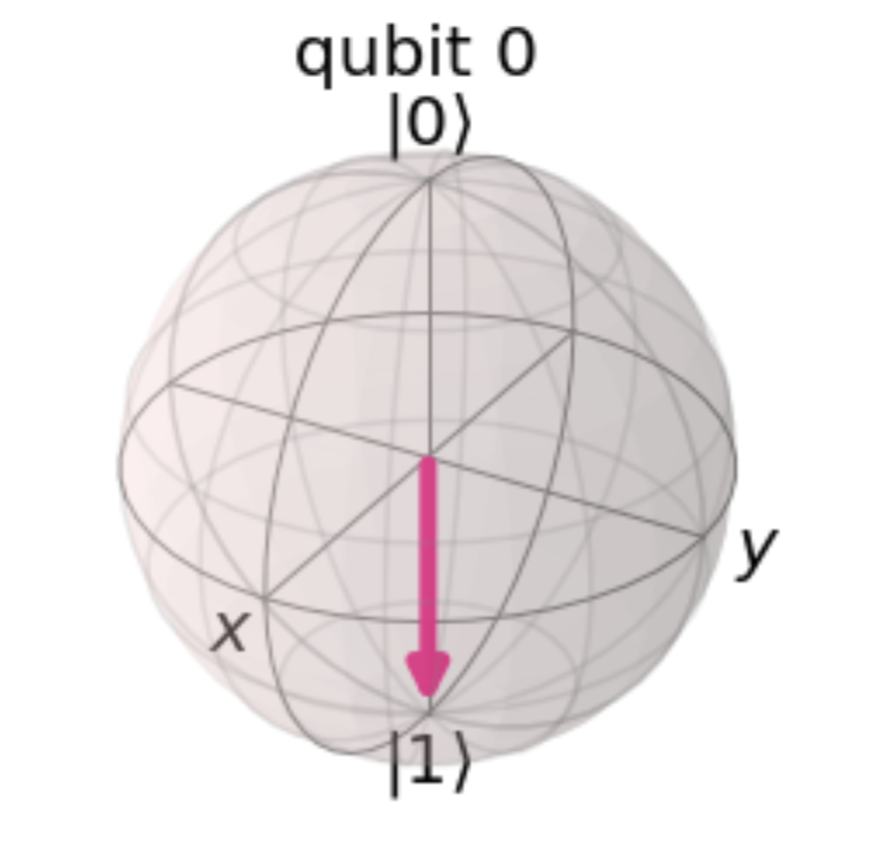
\includegraphics[width=\textwidth]{lab2/images/bSphX2.png}
        \caption{}
        \label{fig:bSphX2}
    \end{subfigure}
    \caption{Bloch sphere showing a) the state of the initialised qubit and b) the state of the qubit after being passed through a Pauli-X gate} 
    \label{fig:bSphereXGate}
\end{figure}

\subsubsection{The Y and Z gates}

Similar to the X gate, the Y and Z Pauli matrices can represent the Y and Z gates in our quantum circuits. These gates perform rotations by $\pi$ around the y and z-axis of the Bloch sphere, respectively.

$$ Y = \begin{bmatrix} 0 & -i \\ i & 0 \end{bmatrix} = -i|0\rangle\langle1| + i|1\rangle\langle0| $$

$$ Z = \begin{bmatrix} 1 & 0 \\ 0 & -1 \end{bmatrix} = |0\rangle\langle0| - |1\rangle\langle1| $$

A circuit was created with an X and Y gate in series, as shown in Figure \ref{fig:xyGateDiagram}.

\begin{figure}[h]
    \centering
    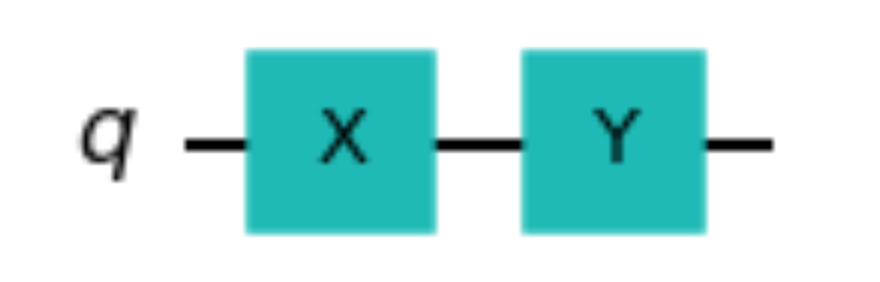
\includegraphics[width=0.3\textwidth]{lab2/images/xyGate.png}
    \caption{Circuit diagram of Pauli-X gate followed by a Pauli-Y gate in series} 
    \label{fig:xyGateDiagram}
\end{figure}

The resultant state was observed through the use of a Bloch sphere. After passing through circuit described in Figure \ref{fig:xyGateDiagram}, the qubit was found to be in state $|0\rangle$ -- seemingly unchanged from its initialised state -- as seen in Figure \ref{fig:xyGateBloc}.

\begin{figure}[h]
    \centering
    \begin{subfigure}[h]{0.33\textwidth}
        \centering
        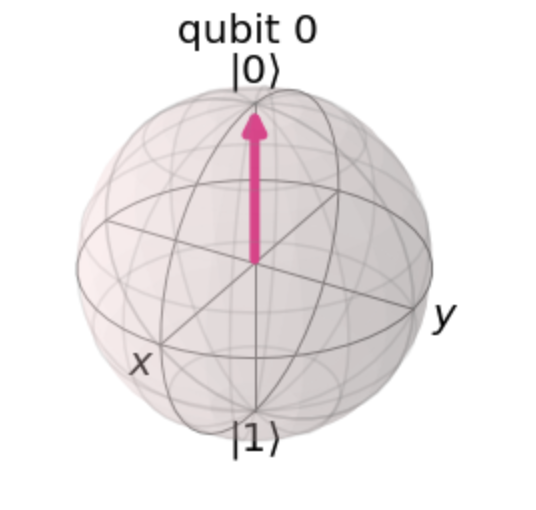
\includegraphics[width=\textwidth]{lab2/images/bSphX1.png}
        \caption{}
        \label{fig:bSphXY1}
    \end{subfigure}
    \hspace{0.2\textwidth}
    \begin{subfigure}[h]{0.33\textwidth}
        \centering
        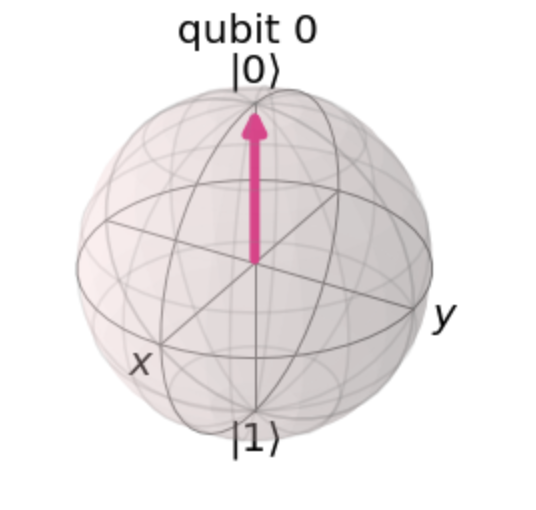
\includegraphics[width=\textwidth]{lab2/images/bSphX1.png}
        \caption{}
        \label{fig:bSphXY2}
    \end{subfigure}
    \caption{Bloch sphere showing a) the state of the initialised qubit and b) the state of the qubit after being passed through a Pauli-X gate and a Pauli-Y gate} 
    \label{fig:xyGateBloc}
\end{figure}

%Need fixed
The explanation for this is as follows:
\begin{enumerate}
    \item The qubit was initialised in state $|0\rangle$
    \item The X gate rotated this state by $\pi$ around the x-axis
    \begin{enumerate}
        \item resulting with a qubit in state $|1\rangle$
    \end{enumerate}
    \item The Y gate then rotated this qubit by $\pi$ around the y-axis
    \begin{enumerate}
        \item resulting in the qubit being in state~$|0\rangle$
    \end{enumerate} 
\end{enumerate}

\subsection{The Hadamard Gate}
The Hadamard gate (H gate) is a fundamental quantum gate, represented by the following matrix:

$$ H = \tfrac{1}{\sqrt{2}}\begin{bmatrix} 1 & 1 \\ 1 & -1 \end{bmatrix} $$

It allows states to occupy a superposition of $|0\rangle$ and $|1\rangle$:

$$ H|0\rangle = \tfrac{1}{\sqrt{2}}\begin{bmatrix} 1 & 1 \\ 1 & -1 \end{bmatrix}\begin{bmatrix} 1 \\ 0 \end{bmatrix} = \tfrac{1}{\sqrt{2}} \begin{bmatrix} 1 \\ 1 \end{bmatrix}= |+\rangle 
\quad \quad \quad \quad 
H|1\rangle = \tfrac{1}{\sqrt{2}}\begin{bmatrix} 1 & 1 \\ 1 & -1 \end{bmatrix}\begin{bmatrix} 0 \\ 1 \end{bmatrix} = \tfrac{1}{\sqrt{2}} \begin{bmatrix} 1 \\ -1 \end{bmatrix}= |-\rangle $$

The H gate can transform the state of the qubit between the X and Z bases. It essentially performs a rotation around the Bloch vector `[1,0,1]' (the line between the x and z-axis).

Applying the sequence of gates: HZH, to any qubit state is equivalent to applying a single X-gate, shown mathematically below.

$$ H = \tfrac{1}{\sqrt{2}}\begin{bmatrix} 1 & 1 \\ 1 & -1 \end{bmatrix} \quad\quad  Z = \begin{bmatrix} 1 & 0 \\ 0 & -1 \end{bmatrix} \quad\quad  X = \begin{bmatrix} 0 & 1 \\ 1 & 0 \end{bmatrix} $$

\begin{equation*} 
\begin{split}
HZH & = \tfrac{1}{\sqrt{2}}\begin{bmatrix} 1 & 1 \\ 1 & -1 \end{bmatrix} \begin{bmatrix} 1 & 0 \\ 0 & -1 \end{bmatrix}\tfrac{1}{\sqrt{2}}\begin{bmatrix} 1 & 1 \\ 1 & -1 \end{bmatrix} \\
HZH & = \tfrac{1}{\sqrt{2}}\tfrac{1}{\sqrt{2}}\begin{bmatrix} 1 & 1 \\ 1 & -1 \end{bmatrix} \begin{bmatrix} 1 & 0 \\ 0 & -1 \end{bmatrix}\begin{bmatrix} 1 & 1 \\ 1 & -1 \end{bmatrix} \\
HZH & = \tfrac{1}{2}\begin{bmatrix} 1 & -1 \\ 1 & 1 \end{bmatrix}\begin{bmatrix} 1 & 1 \\ 1 & -1 \end{bmatrix}\\
HZH & = \tfrac{1}{2}\begin{bmatrix} 0 & 2 \\ 2 & 0 \end{bmatrix} \\
HZH & = \begin{bmatrix} 0 & 1 \\ 1 & 0 \end{bmatrix} \\
HZH & = X
\end{split}
\end{equation*}

The following circuit was written to verify this.

\begin{figure}[h]
    \centering
    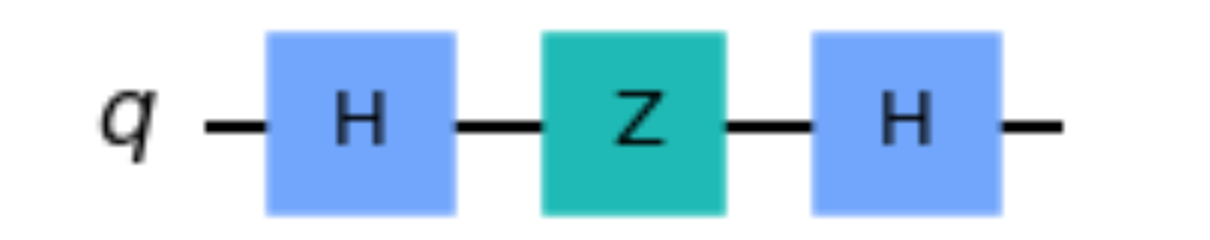
\includegraphics[width=0.4\textwidth]{lab2/images/hzhCircuit.png}
    \caption{Circuit diagram of a Hadamard gate, followed by a Pauli-Z gate, followed by another Hadamard gate in series} 
    \label{fig:hzhCircuit}
\end{figure}

Figure \ref{fig:bSphereHZHGate} shows the resultant state of the qubit after being passed through the circuit shown in Figure \ref{fig:hzhCircuit}.

\begin{figure}[h]
    \centering
    \begin{subfigure}[h]{0.24\textwidth}
        \centering
        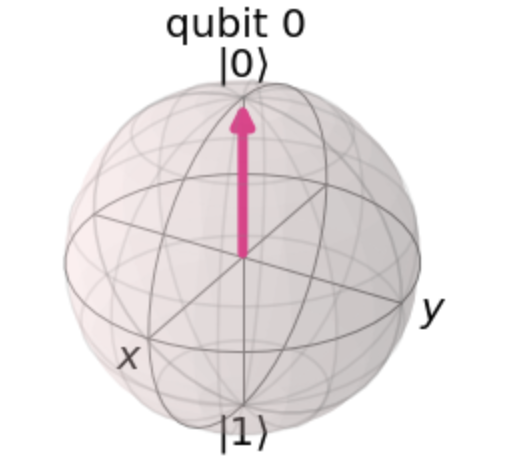
\includegraphics[width=\textwidth]{lab2/images/hzhGate1.png}
        \caption{Initial state}
        \label{fig:hzhGate1}
    \end{subfigure}
    \hfill
    \begin{subfigure}[h]{0.24\textwidth}
        \centering
        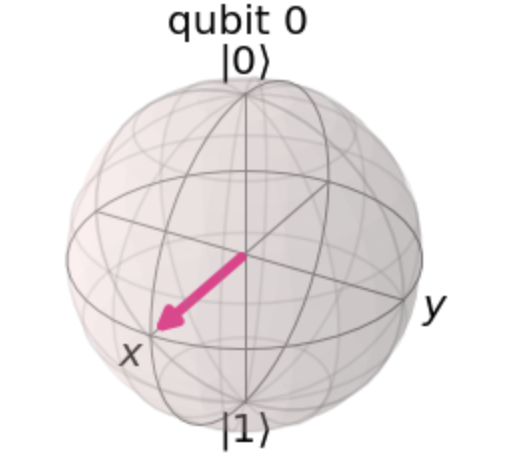
\includegraphics[width=\textwidth]{lab2/images/hzhGate2.png}
        \caption{After H gate}
        \label{fig:hzhGate2}
    \end{subfigure}
        \begin{subfigure}[h]{0.24\textwidth}
        \centering
        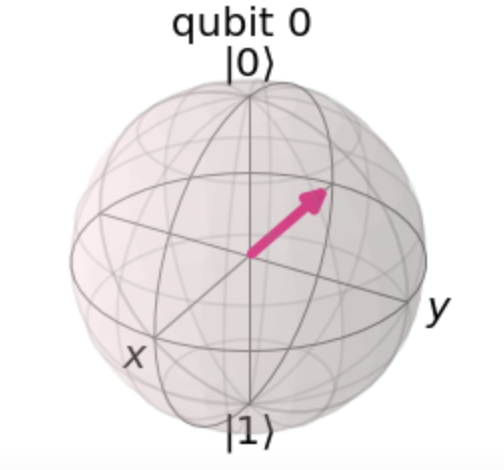
\includegraphics[width=\textwidth]{lab2/images/hzhGate3.png}
        \caption{After Z gate}
        \label{fig:hzhGate3}
    \end{subfigure}
        \begin{subfigure}[h]{0.24\textwidth}
        \centering
        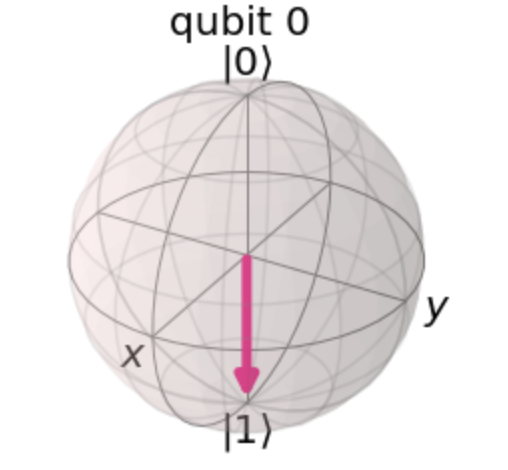
\includegraphics[width=\textwidth]{lab2/images/hzhGate4.png}
        \caption{After H gate}
        \label{fig:hzhGate4}
    \end{subfigure}
    \caption{Bloch sphere showing the state of the qubit after each gate is applied} 
    \label{fig:bSphereHZHGate}
\end{figure}

%FIX?
It is clear upon comparing the initial state (Figure \ref{fig:hzhGate1}) to the final state (Figure \ref{fig:hzhGate4}) that applying the sequence of gates: HZH has an identical effect to applying a single X gate (see Figure \ref{fig:xyGateBloc}).

\subsection{Multi-Qubit Gates}

how to represent the state of a qubit and how to alter those using quantum gates

\subsubsection{The CNOT Gate}
An important two-qubit gate is the CNOT gate. This gate is a conditional gate that performs an X gate on the second qubit (target), if the state of the first qubit (control) is  $|1\rangle$. Table \ref{tab:cNotTruth} shows the truth table for a CNOT gate.

\begin{table}[]
\centering
\begin{tabular}{cccc}
\multicolumn{2}{c}{Input}                         & \multicolumn{2}{c}{Output}   \\ 
\multicolumn{1}{c|}{q1} & \multicolumn{1}{c||}{q2} & \multicolumn{1}{c|}{q1} & q2 \\ \hline\hline
\multicolumn{1}{c|}{0}  & \multicolumn{1}{c||}{0}  & \multicolumn{1}{c|}{0}  & 0  \\ \hline
\multicolumn{1}{c|}{0}  & \multicolumn{1}{c||}{1}  & \multicolumn{1}{c|}{0}  & 1  \\ \hline
\multicolumn{1}{c|}{1}  & \multicolumn{1}{c||}{0}  & \multicolumn{1}{c|}{1}  & 1  \\ \hline
\multicolumn{1}{c|}{1}  & \multicolumn{1}{c||}{1}  & \multicolumn{1}{c|}{1}  & 0 
\end{tabular}
\label{tab:cNotTruth}
\caption{Truth table for CNOT gate}
\end{table}


%q\_1 as the control and q\_2 as the target


A 2-qubit quantum circuit was created, where the 2 qubits are entangled and the output was measured. The circuit diagram is shown in Figure \ref{fig:entangleMeasure}

\begin{figure}[h]
    \centering
    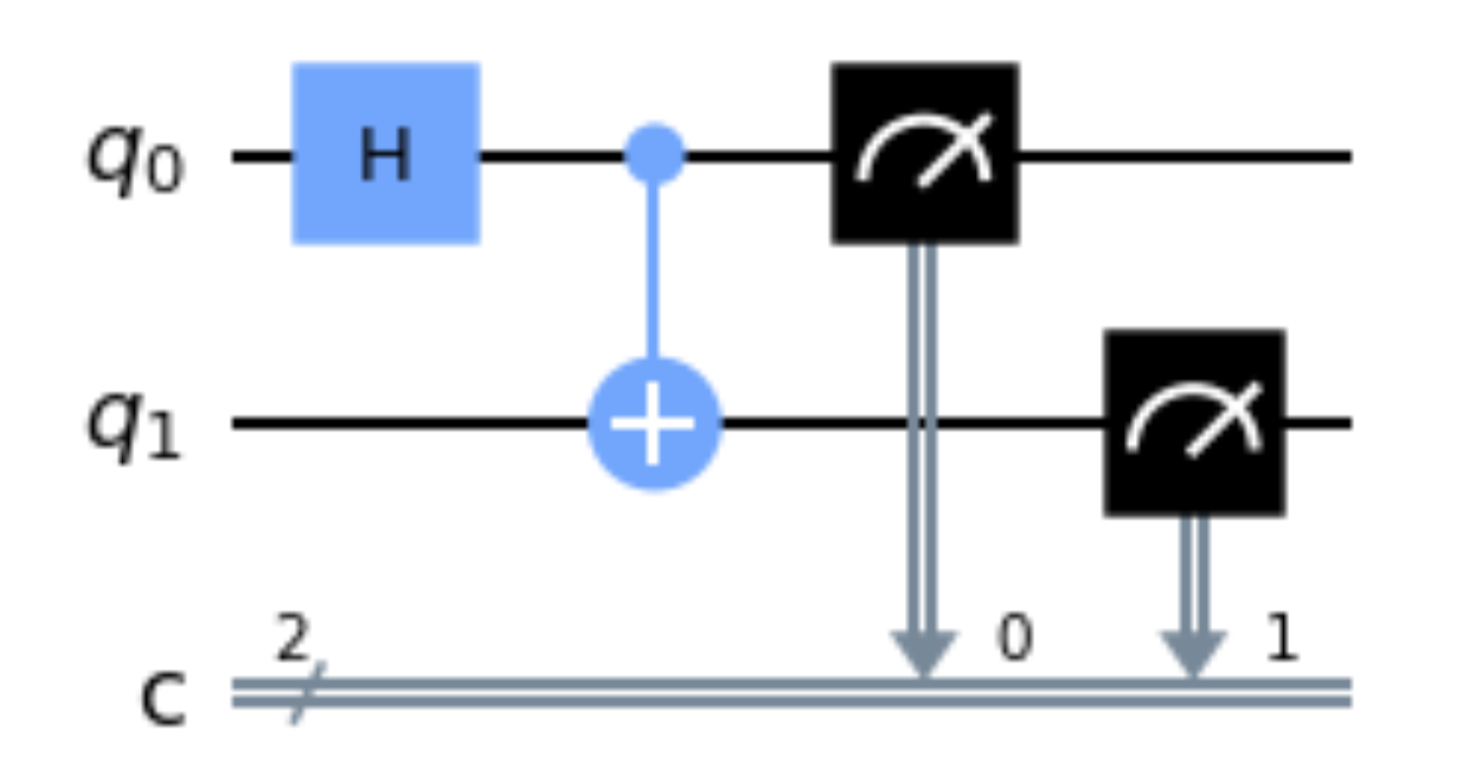
\includegraphics[width=0.4\textwidth]{lab2/images/entangleMeasure.png}
    \caption{entangleMeasure} 
    \label{fig:entangleMeasure}
\end{figure}

So both are initialised as 0. H puts the top in superposition, meaning it is 50\% between 0 and 1. Then when its used as a control bit, its kinda halfway between 0 and 1 meaning half the time it will be a 1 switching the second bit to a 1, then the other half it will be 0 meaning the second qubit will stay 0. As a result, we would expect two possible results from this circuit. Half of the time its 00 and the other half itll be 11. This was circuit was simulated and the results can be found in Figure \ref{fig:qiskitHistogram}.

\begin{figure}[h]
    \centering
    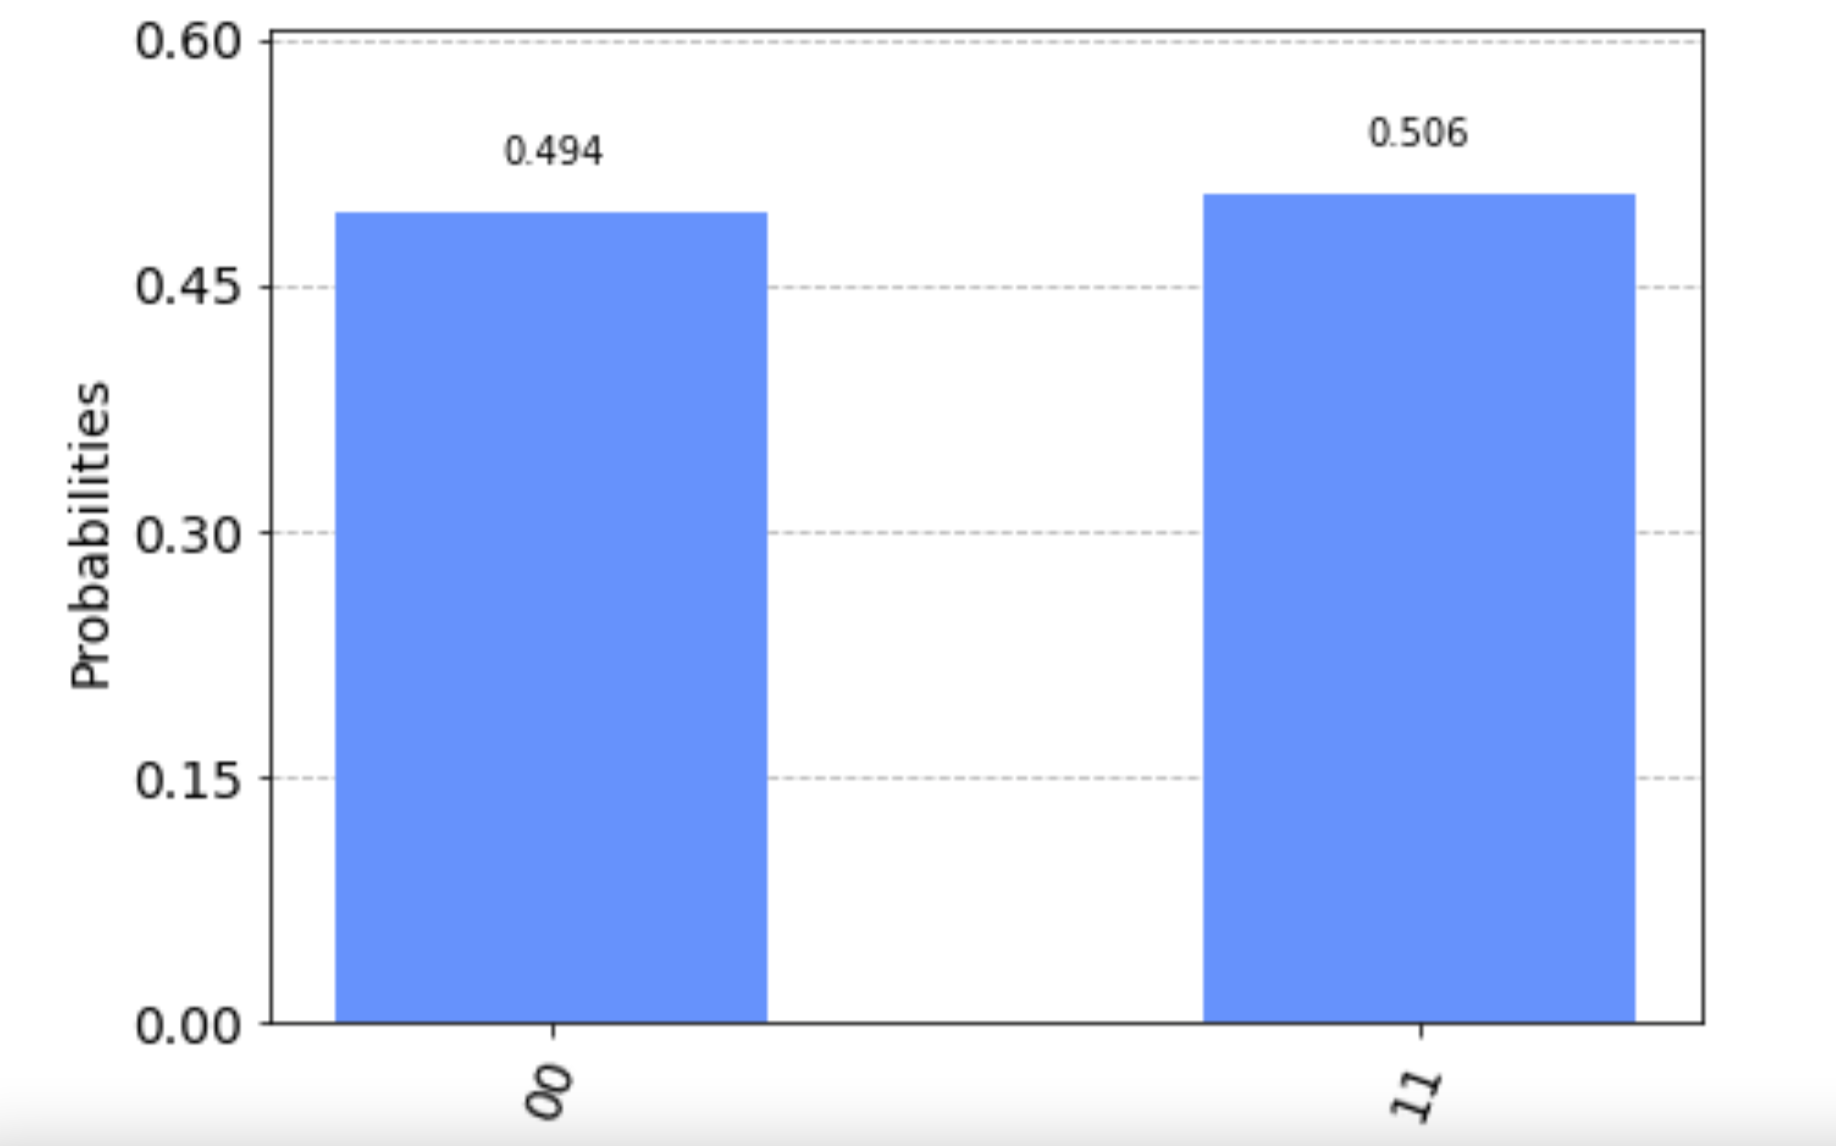
\includegraphics[width=0.75\textwidth]{lab2/images/qiskitHistogram.png}
    \caption{qiskitHistogram} 
    \label{fig:qiskitHistogram}
\end{figure} 

The results show that two 00 and 11 came up which made sense,  however it was not a 50/50 split as expected. This is discussed further in Section \ref{sec:discussion}. To determine a more real response IBMs quantum computer was used. The results can be seen in Figure \ref{fig:ibmHistogram}. Again, there was not a co

\begin{figure}[h]
    \centering
    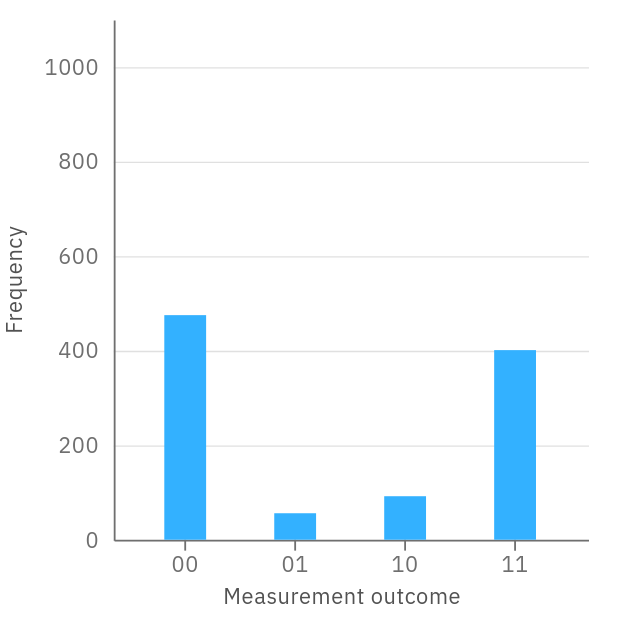
\includegraphics[width=0.4\textwidth]{lab2/images/ibmHistogram.png}
    \caption{qiskitHistogram} 
    \label{fig:ibmHistogram}
\end{figure} 

\section{Comparison of results with theory}
\section{Discussion} \label{sec:discussion}
\textbf{Question 1:}

Initialise a qubit, and apply the X gate to it. Confirm your result by drawing the circuit and visualing the flipped state using the Block sphere (use/copy and paste the examples above wherever appropriate).


\textbf{Question 2:}
Apply the x and y gates to the qubit above and draw it on your screen.

To be frank. That is not a question.

\textbf{Question 3:}
Show mathematically that applying the sequence of gates: HZH, to any qubit state is equivalent to applying an X gate. Then, write a circuit that will show this (you can check each step/rotation, by ploting the new state on the Bloch Sphere each time.


\textbf{Question 4:}
Build a 2-qubit quantum circuit where the 2 qubits are entangled and measure the output. Does this agree with the mathematical prediction? If not, why would you say that is so

\textbf{Question 5:}
Use IBM composer and compare its results to what you obtained above. Are they different? How so? Is there anything you can do to make the results come closer to the mathematica expectation?

\section{Conclusions}